\documentclass[11pt, letterpaper, includehead]{article}

%%%%%%%%%%%%%%%%%%%%% Pre-document %%%%%%%%%%%%%%%%%%%%%
\usepackage{fancyhdr}
\usepackage{float}
\usepackage{array}
\usepackage{nicematrix}
\usepackage{enumitem}
\usepackage{titlesec}
\usepackage{multicol}
\usepackage{scrextend}
\usepackage{hyperref}
\usepackage{amssymb}
\usepackage{amsthm}
\usepackage{tikz}

\setlength{\parindent}{0pt} % Remove auto paragraph indents

% Get rid of those big margins
\usepackage[margin=1in]{geometry}
\newlength\titleindent
\setlength\titleindent{2cm}

\makeatletter
\def\@mathmargin{1in}
\makeatother

\titleformat{\section}[runin]
{\normalfont\bfseries}% formatting commands to apply to the whole heading
{\thesubsection}% the label and number
{0.5em}% space between label/number and subsection title
{}% formatting commands applied just to subsection title
[]% punctuation or other commands following subsection title

\theoremstyle{plain}

\newtheoremstyle{mydefinition}	% Name of the style
{} % Space above
{} % Space below
{\normalfont} % Body font (normal, not bold or italic)
{} % Indent amount
{\itshape} % Theorem head font (italic)
{.} % Punctuation after theorem head
{.5em} % Space after theorem head
{} % Theorem head spec (can be left empty)

\theoremstyle{mydefinition}
\newtheorem{defin}{Definition}

\newtheoremstyle{myproperty}  % Name of the style
{} % Space above
{} % Space below
{\normalfont} % Body font (normal, not bold or italic)
{} % Indent amount
{\itshape} % Theorem head font (italic)
{.} % Punctuation after theorem head
{.5em} % Space after theorem head
{} % Theorem head spec (can be left empty)

\theoremstyle{myproperty}
\newtheorem{prop}{Property}

\begin{document}

\pagestyle{fancy}
% Header
\fancyhead{}
\fancyhead[L]{\textbf{CS23:} Assignment \#4}
\fancyhead[R]{\href{mailto:stepanielh1111@gmail.com}{L'Heureux} \thepage}
% No page numbers for footer
\fancyfoot{}

\begin{center}
    \Large{\textbf{Assignment 4}}\\
    \Large{Graphs}
\end{center}

\begin{enumerate}[label=\textbf{\arabic*}., leftmargin=*]
    \item If 12 people each shake hands with each other, how many handshakes
          took
          place?

          \begin{multicols}{2}
              Let each vertex represent a person, and the edges between them a
              handshake.
              This problem may be represented by a graph of 12 nodes, each of
              degree 11---the
              complete graph $K_{12}$. Each vertex is degree 11, and there are
              12 vertices.
              There are $n(n-1)/2$ edges in graph $K_n$. Therefore, there are
              $12(12-1)/2 = 66$
              edges in graph $K_{12}$. 66 handshakes took place.

              \columnbreak
              \begin{figure}[H]
                  \centering
                  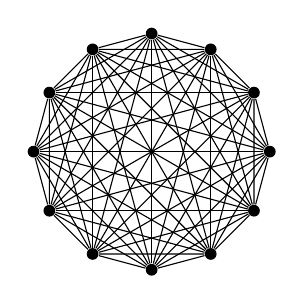
\begin{tikzpicture}[scale=1.5, every node/.style={circle,
                                  fill=black, inner
                                  sep=1.5pt}]
                      \foreach \i in {1,...,12} {
                              \node (N\i) at ({360/12 * (\i - 1)}:1cm) {};
                          }

                      \foreach \i in {1,...,11} {
                              \pgfmathtruncatemacro{\next}{\i+1}
                              \foreach \j in {\next,...,12} {
                                      \draw (N\i) -- (N\j);
                                  }
                          }
                  \end{tikzpicture}
                  \caption{$K_{12}$}
              \end{figure}
          \end{multicols}

    \item In a group of six people, is it possible for everyone to be friends
          with
          exactly two other people in the group? How about three other people?
          Four?

          Let each person be represented by a vertex in a graph, with friendships illustrated as edges between vertices. Note that in any graph, the number of vertices with an odd degree must be even.

          \begin{enumerate}
              \item[$G_1$] Graph of 6 vertices, each of degree 2. The sum of
                  degrees in $G_1$ is $6 \times 2 = 12$. The graph would have 6
                  edges which is
                  possible. Also see Figure \ref{fig:2.G1}.
              \item[$G_2$] Graph of 6 vertices, each of degree 3. The sum of
                  degrees in $G_2$ is $6 \times 3 = 18$. The graph would have 9
                  edges which is
                  possible. Also see Figure \ref{fig:2.G2}.
              \item[$G_3$] Graph of 6 vertices, each of degree 4. The sum of
                  degrees in $G_3$ is $6 \times 4 = 24$. The graph would have
                  12 edges which is
                  possible. Also see Figure \ref{fig:2.G3}.
          \end{enumerate}

          \begin{multicols}{3}

              \begin{figure}[H]
                  \centering
                  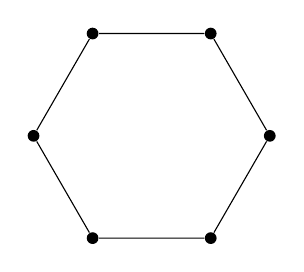
\begin{tikzpicture}[scale=1.5, every node/.style={circle,
                                  fill=black, inner
                                  sep=1.5pt}]
                      \foreach \i in {1,...,6} {
                              \node (N\i) at ({360/6* (\i - 1)}:1cm) {};
                          }

                      \foreach \i/\j in {N1/N2, N2/N3, N3/N4, N4/N5, N5/N6,
                              N6/N1} {
                              \draw (\i) -- (\j);
                          }
                  \end{tikzpicture}
                  \caption{$G_1$}
                  \label{fig:2.G1}
              \end{figure}

              \columnbreak

              \begin{figure}[H]
                  \centering
                  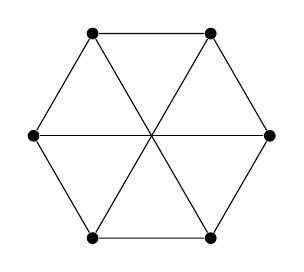
\begin{tikzpicture}[scale=1.5, every node/.style={circle,
                                  fill=black, inner
                                  sep=1.5pt}]
                      \foreach \i in {1,...,6} {
                              \node (N\i) at ({360/6* (\i - 1)}:1cm) {};
                          }

                      \foreach \i/\j in {N1/N2, N2/N3, N3/N4, N4/N5, N5/N6, N6/N1,
                              N1/N4, N2/N5, N3/N6} {
                              \draw (\i) -- (\j);
                          }
                  \end{tikzpicture}
                  \caption{$G_2$}
                  \label{fig:2.G2}
              \end{figure}

              \columnbreak

              \begin{figure}[H]
                  \centering
                  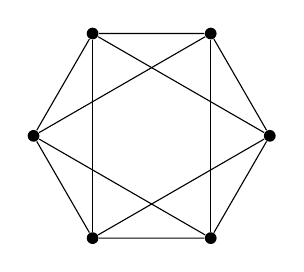
\begin{tikzpicture}[scale=1.5, every node/.style={circle,
                                  fill=black, inner
                                  sep=1.5pt}]
                      \foreach \i in {1,...,6} {
                              \node (N\i) at ({360/6* (\i - 1)}:1cm) {};
                          }

                      \foreach \i/\j in {N1/N2, N2/N3, N3/N4, N4/N5, N5/N6, N6/N1,
                              N1/N3, N2/N4, N5/N1, N6/N4, N6/N2, N5/N3} {
                              \draw (\i) -- (\j);
                          }
                  \end{tikzpicture}
                  \caption{$G_3$}
                  \label{fig:2.G3}
              \end{figure}

          \end{multicols}
    \item Is it possible for two graphs with the same number of nodes and edges
          to not be isomorphic? What if the degrees of the nodes in the two
          graphs
          are the same? Give example graphs or explain why.

          Two graphs are isomorphic if there is a one-to-one relationship
          (bijection) between their vertices that preserves adjacency---that is, the
          graphs have the same structure and differ only in the labeling of their
          vertices.

          Graphs $G_1$ (\ref{fig:3.G1}) and $G_2$ (\ref{fig:3.G2}) have $|E| =
              5$ and $|V| = 5$. E is not reachable in $G_1$, however every node is reachable
          in $G_2$, therefore they cannot be isomorphic.

          Graphs $G_2$ (\ref{fig:3.G3}) and $G_4$ (\ref{fig:3.G4}) have $|E| =
              6$, $|V| = 5$, and degree sequence (3, 3, 2, 2, 2). For $G_3$ and $G_4$ to be
          isomorphic, there must exist a bijective mapping between the vertices which
          preserves adjacency. This implies that vertices with the same degree must be
          mapped to each other. In $G_3$, vertices A and B are degree three and are
          adjacent. In $G_4$ vertices X and V are degree three but are not adjacent.
          Therefore, the graphs cannot be isomorphic.
          \begin{multicols}{4}

              \begin{figure}[H]
                  \centering
                  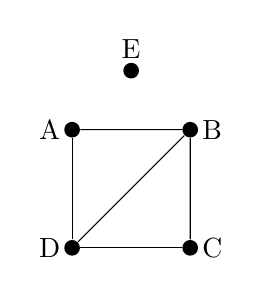
\begin{tikzpicture}[scale=1.5, every node/.style={circle,
                                  fill=black,
                                  inner sep=2pt}]

                      \node (u) at (0, 1) {};
                      \node (v) at (1, 1) {};
                      \node (w) at (1, 0) {};
                      \node (x) at (0, 0) {};
                      \node (y) at (0.5, 1.5) {};

                      \node[draw=none, fill=none, anchor=east] at (u) {A};
                      \node[draw=none, fill=none, anchor=west] at (v) {B};
                      \node[draw=none, fill=none, anchor=west] at (w) {C};
                      \node[draw=none, fill=none, anchor=east] at (x) {D};
                      \node[draw=none, fill=none, anchor=south] at (y) {E};

                      \foreach \i/\j in {u/v, v/w, w/x, x/u, v/x} {
                              \draw (\i) -- (\j);
                          }
                  \end{tikzpicture}
                  \caption{$G_1$}
                  \label{fig:3.G1}
              \end{figure}

              \columnbreak

              \begin{figure}[H]
                  \centering
                  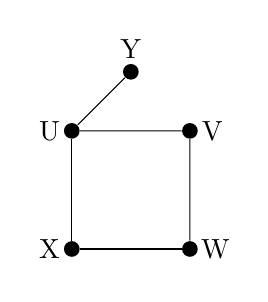
\begin{tikzpicture}[scale=1.5, every node/.style={circle,
                                  fill=black,
                                  inner sep=2pt}]
                      \node (u) at (0, 1) {};
                      \node (v) at (1, 1) {};
                      \node (w) at (1, 0) {};
                      \node (x) at (0, 0) {};
                      \node (y) at (0.5, 1.5) {};

                      \node[draw=none, fill=none, anchor=east] at (u) {U};
                      \node[draw=none, fill=none, anchor=west] at (v) {V};
                      \node[draw=none, fill=none, anchor=west] at (w) {W};
                      \node[draw=none, fill=none, anchor=east] at (x) {X};
                      \node[draw=none, fill=none, anchor=south] at (y) {Y};

                      \foreach \i/\j in {u/v, v/w, w/x, x/u, u/y} {
                              \draw (\i) -- (\j);
                          }
                  \end{tikzpicture}
                  \caption{$G_2$}
                  \label{fig:3.G2}
              \end{figure}

              \columnbreak

              \begin{figure}[H]
                  \centering
                  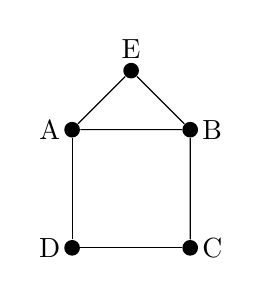
\begin{tikzpicture}[scale=1.5, every node/.style={circle,
                                  fill=black,
                                  inner
                                  sep=2pt}]
                      \node (u) at (0, 1) {};
                      \node (v) at (1, 1) {};
                      \node (w) at (1, 0) {};
                      \node (x) at (0, 0) {};
                      \node (y) at (0.5, 1.5) {};

                      \node[draw=none, fill=none, anchor=east] at (u) {A};
                      \node[draw=none, fill=none, anchor=west] at (v) {B};
                      \node[draw=none, fill=none, anchor=west] at (w) {C};
                      \node[draw=none, fill=none, anchor=east] at (x) {D};
                      \node[draw=none, fill=none, anchor=south] at (y) {E};

                      \foreach \i/\j in {u/v, v/w, w/x, x/u, u/y, v/y} {
                              \draw (\i) -- (\j);
                          }
                  \end{tikzpicture}
                  \caption{$G_3$}
                  \label{fig:3.G3}
              \end{figure}

              \columnbreak

              \begin{figure}[H]
                  \centering
                  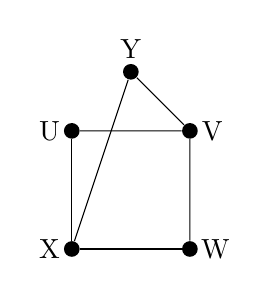
\begin{tikzpicture}[scale=1.5, every node/.style={circle,
                                  fill=black,
                                  inner
                                  sep=2pt}]
                      \centering
                      \node (u) at (0, 1) {};
                      \node (v) at (1, 1) {};
                      \node (w) at (1, 0) {};
                      \node (x) at (0, 0) {};
                      \node (y) at (0.5, 1.5) {};

                      \node[draw=none, fill=none, anchor=east] at (u) {U};
                      \node[draw=none, fill=none, anchor=west] at (v) {V};
                      \node[draw=none, fill=none, anchor=west] at (w) {W};
                      \node[draw=none, fill=none, anchor=east] at (x) {X};
                      \node[draw=none, fill=none, anchor=south] at (y) {Y};

                      \foreach \i/\j in {u/v, v/w, w/x, x/u, v/y, y/x} {
                              \draw (\i) -- (\j);
                          }
                  \end{tikzpicture}
                  \caption{$G_4$}
                  \label{fig:3.G4}
              \end{figure}

          \end{multicols}

    \item What is the largest number of edges possible in a graph with 10
          vertices?
          What is the largest number of edges possible in a bipartite graph 
          with 10
          vertices? What is the largest number of edges possible in a tree with
          10
          vertices?

          \begin{enumerate}
            \item[(a)] The largest number of edges in a graph with 10 vertices is the complete graph $K_{10}$ with $|E| = 10(10-1)/2 = 45$.
            \item[(b)] The largest number of edges in a bipartite graph with 10 vertices will be a complete bipartite graph $K_{m, n}$ such that $m + n = 10$. The number of edges in a complete bipartite graph is $m \times n$ by the Handshake Lemma. Therefore the constraint $m + n = 10$, we wish to maximize $m \times n$.
            
            Let 
        \[
        f(m, n) = mn \quad \text{and} \quad g(m, n) = m + n - 10.
        \]

        Using the method of Lagrange multipliers:
        \[
        \nabla f(m, n) = \langle n, m \rangle, \quad \nabla g(m, n) = \langle 1, 1 \rangle.
        \]

        \[
        \nabla f = \lambda \nabla g \Rightarrow 
        \begin{cases}
        n = \lambda, \\
        m = \lambda,
        \end{cases}
        \Rightarrow m = n.
        \]

        Substitute into the constraint:
        \[
        m + n = 10 \Rightarrow 2m = 10 \Rightarrow m = 5.
        \]

        Because $m = n$ then:
        \[
        m = 5 \Rightarrow n = 5.
        \]

            The bipartite graph with 10 vertices and the most possible edges is $K_{5, 5}$, which has 25 edges.
            \item[(c)] In any tree, the number of edges is given by $|E| = |V|-1$. In a tree with 10 vertices, the number of edges is therefore $|E| = 10-1 = 9$.
          \end{enumerate}
    \item Consider graphs with $n$ vertices. Remember, graphs do not need to be
          \emph{connected}.
          \begin{enumerate}[leftmargin=*]
              \item[(a)] How many edges must the graph have to guarantee at
                  least one vertex
                  has degree two or more. Prove your answer.

                  \begin{proof}

                    By direct proof.

                    Let $G$ be a graph with $|V| = n$. 
                    
                    The maximum number of edges $G$ can have while no vertex has degree 2 is achieved when every vertex has degree exactly 1.

                    By the Handshake Lemma, the total number of edges in a graph is given by:

                    \[
                    \sum_{v \in V} d(v) = 2e \quad \Rightarrow \quad e = \frac{1}{2} \sum_{v \in V} d(v)
                    \]

                    Since every vertex has degree 1, the sum of the degrees is:
                    \[
                    \sum_{i=1}^{n} 1 = n \quad \Rightarrow \quad e = \left\lfloor \frac{n}{2} \right\rfloor
                    \]

                    Now, suppose we add one more edge to this graph. This edge must connect to at least one existing vertex, increasing its degree to 2.
                
                    Therefore, $G$ must have $\lfloor \frac{n}{2} \rfloor + 1$ edges to guarantee at
                    least one vertex has degree two or greater.
                  \end{proof}

              \item[(b)] How many edges must the graph have to guarantee all vertices
                  have degree two or more? Prove your answer.


                \begin{proof} By direct proof.

                    Let $G$ be a graph with $|V| = n$.

                    The maximum number of edges $G$ can have while one vertex $v$ is disconnected occurs when when the remaining $n - 1$ vertices form a complete subgraph $ K_{n-1} $. This subgraph has:
                    
                    
                    \[
                    e = \frac{(n - 1)(n - 2)}{2}
                    \]
                    
                    Every vertex in $ K_{n-1} $ has degree $ n - 2 $, which is at least 2 for all $ n \geq 4 $.
                    
                    Now, add one edge connecting $ v $ to a vertex $ u \in K_{n-1} $, so that $v$ has degree 1. The total number of edges is now:
                    
                    \[
                    e = \frac{(n - 1)(n - 2)}{2} + 1.
                    \]
                                        
                    Now, add one more edge connecting $ v $ to another vertex $ w \in K_{n-1} $, so that $ v $ is now adjacent to two vertices.
                    
                    Therefore $ \deg(v) = 2 $ and all other vertices still have degree at least $ n - 2 $ because edges were never removed. 
                    
                    The minimum total number of edges is then:
                    \[
                    e = \frac{(n - 1)(n - 2)}{2} + 2.
                    \]

                    $G$ must have $\frac{(n - 1)(n - 2)}{2} + 2$ to guarantee all vertices have degree two or more.
                    
                    \end{proof}
                    
          \end{enumerate}
        
    \item Which of the graphs below are bipartite? Justify your answers.
    
    $G_1$ (\ref{fig:6.G1}), $G_2$ (\ref{fig:6.G2}), and $G_4$ (\ref{fig:6.G4}) are bipartite. $G_3$ (\ref{fig:6.G3}) is not bipartite.
    
    \begin{multicols}{4}
        \vspace*{\fill}
        \begin{figure}[H]
            \centering
            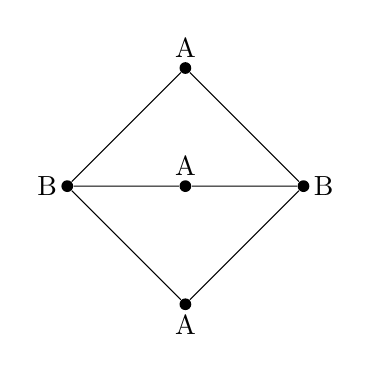
\begin{tikzpicture}[scale=1.5, every node/.style={circle,
                fill=black,
                inner
                sep=1.5pt}]
            \node (1) at (0.5, 0) {};
            \node (2) at (0.5, 2) {};
            \node (3) at (1.5, 1) {};
            \node (4) at (-0.5, 1) {};
            \node (5) at (0.5, 1) {};

            \node[draw=none, fill=none, anchor=north] at (1) {A};
            \node[draw=none, fill=none, anchor=south] at (2) {A};
            \node[draw=none, fill=none, anchor=west] at (3) {B};
            \node[draw=none, fill=none, anchor=east] at (4) {B};
            \node[draw=none, fill=none, anchor=south] at (5) {A};

            \foreach \i/\j in {3/5, 4/5, 2/3, 1/4, 1/3, 4/2} {
                    \draw (\i) -- (\j);
                }
        \end{tikzpicture}
            \caption{$G_1$}
            \label{fig:6.G1}
        \end{figure}

        \columnbreak
        \vspace*{\fill}

        \begin{figure}[H]
            \centering
            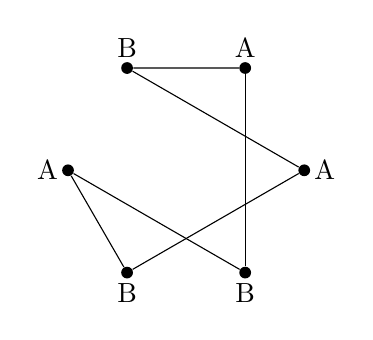
\begin{tikzpicture}[scale=1.5, every node/.style={circle,
                            fill=black, inner
                            sep=1.5pt}]
                \foreach \i in {1,...,6} {
                        \node (N\i) at ({360/6* (\i - 1)}:1cm) {};
                    }

                \foreach \i/\j in {N4/N5, N3/N2,
                        N1/N3, N5/N1, N6/N4, N6/N2} {
                        \draw (\i) -- (\j);
                    }
                    \node[draw=none, fill=none, anchor=west]    at (N1) {A};
                    \node[draw=none, fill=none, anchor=south]   at (N2) {A};
                    \node[draw=none, fill=none, anchor=south]   at (N3) {B};
                    \node[draw=none, fill=none, anchor=north]   at (N6) {B};
                    \node[draw=none, fill=none, anchor=east]    at (N4) {A};
                    \node[draw=none, fill=none, anchor=north]   at (N5) {B};
            \end{tikzpicture}
            \caption{$G_2$}
            \label{fig:6.G2}
        \end{figure}

        \columnbreak
        \vspace*{\fill}
    
        \begin{figure}[H]
            \centering
            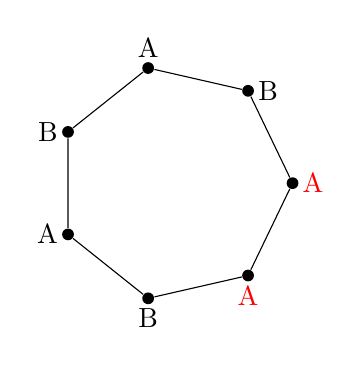
\begin{tikzpicture}[scale=1.5, every node/.style={circle,
                            fill=black, inner
                            sep=1.5pt}]
                \foreach \i in {1,...,7} {
                        \node (N\i) at ({360/7* (\i - 1)}:1cm) {};
                    }

                    \foreach \i in {1,...,6} {
                        \pgfmathtruncatemacro{\next}{\i+1}
                        \draw (N\i) -- (N\next);
                    }
                    \draw (N1) -- (N7);

                    \node[draw=none, fill=none, text=red, anchor=west]    at (N1) {A};
                    \node[draw=none, fill=none, anchor=west]    at (N2) {B};
                    \node[draw=none, fill=none, anchor=south]   at (N3) {A};
                    \node[draw=none, fill=none, anchor=east]    at (N4) {B};
                    \node[draw=none, fill=none, anchor=east]    at (N5) {A};
                    \node[draw=none, fill=none, anchor=north]   at (N6) {B};
                    \node[draw=none, fill=none, text=red, anchor=north]   at (N7) {A};
                
            \end{tikzpicture}
            \caption{$G_3$}
            \label{fig:6.G3}
        \end{figure}

        \columnbreak
        \vspace*{\fill}

        \begin{figure}[H]
            \centering
            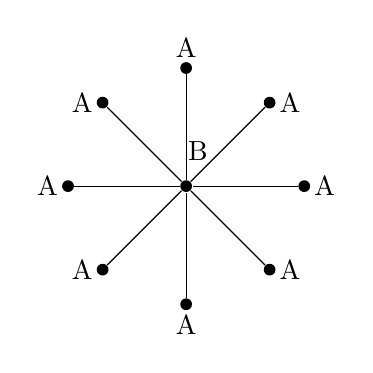
\begin{tikzpicture}[scale=1.5, every node/.style={circle,
                            fill=black, inner
                            sep=1.5pt}]
                \foreach \i in {1,...,8} {
                        \node (N\i) at ({360/8* (\i - 1)}:1cm) {};
                    }
                
                \node (N9) at (0,0) {};
               
                \foreach \i in {1,...,8} {
                        \draw (N\i) -- (N9);
                }
                
                \node[draw=none, fill=none, anchor=west]    at (N8) {A};
                \node[draw=none, fill=none, anchor=west]    at (N1) {A};
                \node[draw=none, fill=none, anchor=west]    at (N2) {A};
                \node[draw=none, fill=none, anchor=south]   at (N3) {A};
                \node[draw=none, fill=none, anchor=east]    at (N4) {A};
                \node[draw=none, fill=none, anchor=east]    at (N5) {A};
                \node[draw=none, fill=none, anchor=east]    at (N6) {A};
                \node[draw=none, fill=none, anchor=north]   at (N7) {A};
                \node[draw=none, fill=none]                 at (0.1, 0.3) {B};
            \end{tikzpicture}
            \caption{$G_4$}
            \label{fig:6.G4}
        \end{figure}

    \end{multicols}

\end{enumerate}

\end{document}